%LaTex Template Authors:
%	Kevin Turkington
%	Mark Bereza
%	Joseph Struth


\documentclass[onecolumn, draftclsnofoot, 10pt, compsoc]{IEEEtran}
%imported packages
\usepackage{hyperref}
\usepackage{graphicx}
\usepackage{geometry}
\usepackage{caption}
\usepackage{float}
%documentation for math: https://en.wikibooks.org/wiki/LaTeX/Mathematics
\usepackage{amsmath} %equations are done with this package
%for tables use tabular
\captionsetup{justification=centering}
%page settings
\geometry{textheight=9.5in, textwidth=7in}
\hypersetup{pdfauthor={nxkryptor},
	pdftitle={OSU USLI},
	pdfsubject={ME},
	pdfkeywords={},
	pdfproducer={Latex with hyperref, or other system},
	pdfcreator={pdflatex, or other tool}
}


%title page
\begin{document}% <<< START WRITING HERE
\tableofcontents
\listoffigures
\listoftables

%ONLY WTIE THINGS IN text.tex
\section{sectioning example}
Lorem ipsum dolor sit amet, consectetur adipiscing elit. Pellentesque elit nisl, mollis non blandit eu, lobortis a ex. Nullam et urna venenatis velit sollicitudin rutrum in ut ligula. Vivamus eget metus lorem. Integer id ligula interdum, luctus orci at, elementum risus. Nunc lobortis enim vitae nulla vehicula, quis tristique nisl faucibus. Donec imperdiet turpis metus, fringilla volutpat tortor ultrices sit amet.
\subsection{ipsum}
Lorem ipsum dolor sit amet, consectetur adipiscing elit. Pellentesque elit nisl, mollis non blandit eu, lobortis a ex.
\subsubsection{dolor}
Lorem ipsum dolor sit amet, consectetur adipiscing elit. Pellentesque elit nisl, mollis non blandit eu, lobortis a ex. Nullam et urna venenatis velit sollicitudin rutrum in ut ligula. Vivamus eget metus lorem. Integer id ligula interdum, luctus orci at, elementum risus. 

\newpage %forces a new page
\section{examples}
\subsection{quoting stuff}
something im quoting here\cite{USLI_handbook}

\subsection{lists}

\subsubsection{unordered list}
\begin{itemize}
\item thing 1
\item thing 2
\end{itemize}

\subsubsection{ordered list}
\begin{enumerate}
\item thing 1
\item thing 2
\end{enumerate}

\subsection{pictures}
\begin{figure}[H]
	\centering
	
\includegraphics[width=.9\linewidth]{meme.jpg}
	\caption{we get it nasa...}
\end{figure}

\begin{figure}[H]
	\centering
	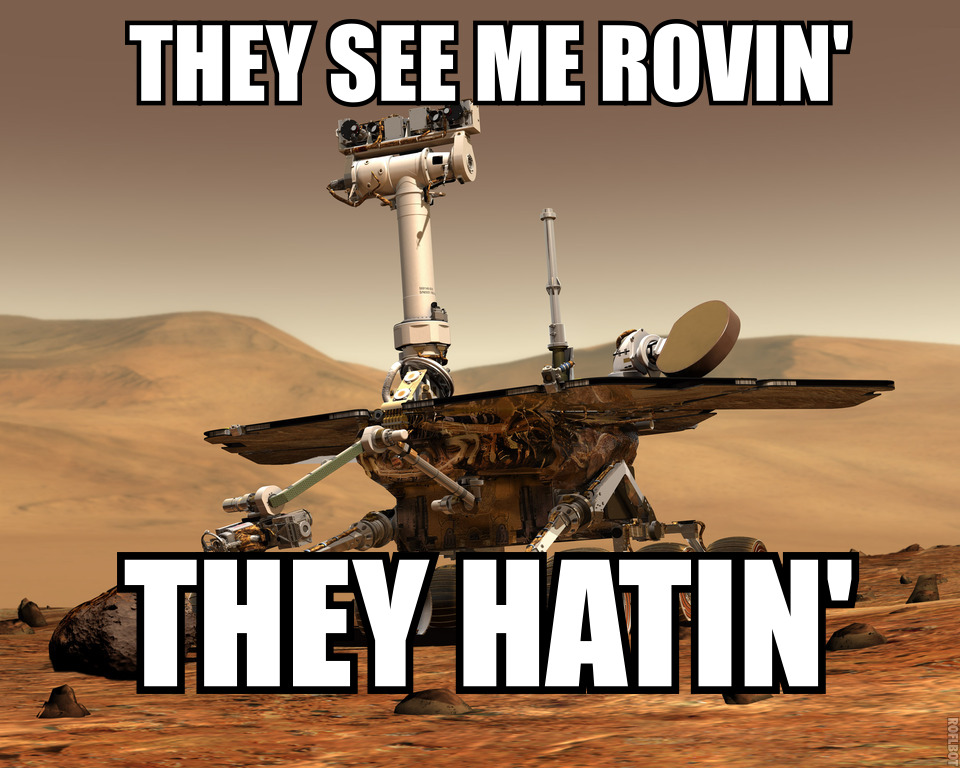
\includegraphics[width=.9\linewidth]{rover.jpg}
	\caption{they rollin}
\end{figure}

\subsection{tables}
if you have a complex table import it as a picture
\\% <<< this acts as a new line

% Documentation: https://en.wikibooks.org/wiki/LaTeX/Tables
\begin{table}[hp]
\centering
\begin{tabular} {l p{0.45\linewidth} p{0.45\linewidth}} \textbf{Week} & \textbf{Work Done} & \textbf{Problems Encountered}\\\hline
item 1 & item 2 & item 3 \\
item 1 & item 2 & item 3 \\
\end{tabular}
\caption{this is my table}
\end{table}

\subsection{math equations}

\[
e^{\pi i} + 1 = 0
\]

\[
x^n + y^n = z^n
\]

\section{how to compile your document}
\subsection{web}
this is the suggested way to compile your document as www.overleaf.com shows where your error is,
and contains a point and click feature for editing, and has autocorrect.
\subsection{desktop}
this is the second easiest way is to use visual studio code with the following extensions
\begin{itemize}
	\item LaTex language support (syntax highlighting)
	\item LaTex Workshop (easy compiling without makefile)
\end{itemize}



\newpage %forces a new page
% bibliography
\nocite{*}%if nothing is referenced it will still show up in refs
\bibliographystyle{plain}
\bibliography{main}
%end bibliography

\end{document}